% Options for packages loaded elsewhere
\PassOptionsToPackage{unicode}{hyperref}
\PassOptionsToPackage{hyphens}{url}
%
\documentclass[
  14pt,
  ignorenonframetext,
  aspectratio=169,
]{beamer}
\usepackage{pgfpages}
\setbeamertemplate{caption}[numbered]
\setbeamertemplate{caption label separator}{: }
\setbeamercolor{caption name}{fg=normal text.fg}
\beamertemplatenavigationsymbolsempty
% Prevent slide breaks in the middle of a paragraph
\widowpenalties 1 10000
\raggedbottom

\usepackage{amsmath,amssymb}
\usepackage{iftex}
\ifPDFTeX
  \usepackage[T1]{fontenc}
  \usepackage[utf8]{inputenc}
  \usepackage{textcomp} % provide euro and other symbols
\else % if luatex or xetex
  \usepackage{unicode-math}
  \defaultfontfeatures{Scale=MatchLowercase}
  \defaultfontfeatures[\rmfamily]{Ligatures=TeX,Scale=1}
\fi
\usepackage{lmodern}
\ifPDFTeX\else  
    % xetex/luatex font selection
\fi
% Use upquote if available, for straight quotes in verbatim environments
\IfFileExists{upquote.sty}{\usepackage{upquote}}{}
\IfFileExists{microtype.sty}{% use microtype if available
  \usepackage[]{microtype}
  \UseMicrotypeSet[protrusion]{basicmath} % disable protrusion for tt fonts
}{}
\makeatletter
\@ifundefined{KOMAClassName}{% if non-KOMA class
  \IfFileExists{parskip.sty}{%
    \usepackage{parskip}
  }{% else
    \setlength{\parindent}{0pt}
    \setlength{\parskip}{6pt plus 2pt minus 1pt}}
}{% if KOMA class
  \KOMAoptions{parskip=half}}
\makeatother
\usepackage{xcolor}
\newif\ifbibliography
\setlength{\emergencystretch}{3em} % prevent overfull lines
\setcounter{secnumdepth}{-\maxdimen} % remove section numbering

\usepackage{color}
\usepackage{fancyvrb}
\newcommand{\VerbBar}{|}
\newcommand{\VERB}{\Verb[commandchars=\\\{\}]}
\DefineVerbatimEnvironment{Highlighting}{Verbatim}{commandchars=\\\{\}}
% Add ',fontsize=\small' for more characters per line
\usepackage{framed}
\definecolor{shadecolor}{RGB}{248,248,248}
\newenvironment{Shaded}{\begin{snugshade}}{\end{snugshade}}
\newcommand{\AlertTok}[1]{\textcolor[rgb]{0.94,0.16,0.16}{#1}}
\newcommand{\AnnotationTok}[1]{\textcolor[rgb]{0.56,0.35,0.01}{\textbf{\textit{#1}}}}
\newcommand{\AttributeTok}[1]{\textcolor[rgb]{0.13,0.29,0.53}{#1}}
\newcommand{\BaseNTok}[1]{\textcolor[rgb]{0.00,0.00,0.81}{#1}}
\newcommand{\BuiltInTok}[1]{#1}
\newcommand{\CharTok}[1]{\textcolor[rgb]{0.31,0.60,0.02}{#1}}
\newcommand{\CommentTok}[1]{\textcolor[rgb]{0.56,0.35,0.01}{\textit{#1}}}
\newcommand{\CommentVarTok}[1]{\textcolor[rgb]{0.56,0.35,0.01}{\textbf{\textit{#1}}}}
\newcommand{\ConstantTok}[1]{\textcolor[rgb]{0.56,0.35,0.01}{#1}}
\newcommand{\ControlFlowTok}[1]{\textcolor[rgb]{0.13,0.29,0.53}{\textbf{#1}}}
\newcommand{\DataTypeTok}[1]{\textcolor[rgb]{0.13,0.29,0.53}{#1}}
\newcommand{\DecValTok}[1]{\textcolor[rgb]{0.00,0.00,0.81}{#1}}
\newcommand{\DocumentationTok}[1]{\textcolor[rgb]{0.56,0.35,0.01}{\textbf{\textit{#1}}}}
\newcommand{\ErrorTok}[1]{\textcolor[rgb]{0.64,0.00,0.00}{\textbf{#1}}}
\newcommand{\ExtensionTok}[1]{#1}
\newcommand{\FloatTok}[1]{\textcolor[rgb]{0.00,0.00,0.81}{#1}}
\newcommand{\FunctionTok}[1]{\textcolor[rgb]{0.13,0.29,0.53}{\textbf{#1}}}
\newcommand{\ImportTok}[1]{#1}
\newcommand{\InformationTok}[1]{\textcolor[rgb]{0.56,0.35,0.01}{\textbf{\textit{#1}}}}
\newcommand{\KeywordTok}[1]{\textcolor[rgb]{0.13,0.29,0.53}{\textbf{#1}}}
\newcommand{\NormalTok}[1]{#1}
\newcommand{\OperatorTok}[1]{\textcolor[rgb]{0.81,0.36,0.00}{\textbf{#1}}}
\newcommand{\OtherTok}[1]{\textcolor[rgb]{0.56,0.35,0.01}{#1}}
\newcommand{\PreprocessorTok}[1]{\textcolor[rgb]{0.56,0.35,0.01}{\textit{#1}}}
\newcommand{\RegionMarkerTok}[1]{#1}
\newcommand{\SpecialCharTok}[1]{\textcolor[rgb]{0.81,0.36,0.00}{\textbf{#1}}}
\newcommand{\SpecialStringTok}[1]{\textcolor[rgb]{0.31,0.60,0.02}{#1}}
\newcommand{\StringTok}[1]{\textcolor[rgb]{0.31,0.60,0.02}{#1}}
\newcommand{\VariableTok}[1]{\textcolor[rgb]{0.00,0.00,0.00}{#1}}
\newcommand{\VerbatimStringTok}[1]{\textcolor[rgb]{0.31,0.60,0.02}{#1}}
\newcommand{\WarningTok}[1]{\textcolor[rgb]{0.56,0.35,0.01}{\textbf{\textit{#1}}}}

\providecommand{\tightlist}{%
  \setlength{\itemsep}{0pt}\setlength{\parskip}{0pt}}\usepackage{longtable,booktabs,array}
\usepackage{calc} % for calculating minipage widths
\usepackage{caption}
% Make caption package work with longtable
\makeatletter
\def\fnum@table{\tablename~\thetable}
\makeatother
\usepackage{graphicx}
\makeatletter
\newsavebox\pandoc@box
\newcommand*\pandocbounded[1]{% scales image to fit in text height/width
  \sbox\pandoc@box{#1}%
  \Gscale@div\@tempa{\textheight}{\dimexpr\ht\pandoc@box+\dp\pandoc@box\relax}%
  \Gscale@div\@tempb{\linewidth}{\wd\pandoc@box}%
  \ifdim\@tempb\p@<\@tempa\p@\let\@tempa\@tempb\fi% select the smaller of both
  \ifdim\@tempa\p@<\p@\scalebox{\@tempa}{\usebox\pandoc@box}%
  \else\usebox{\pandoc@box}%
  \fi%
}
% Set default figure placement to htbp
\def\fps@figure{htbp}
\makeatother


% Tikz plots

\usepackage{tikz}
\usepackage{forest}

\usetikzlibrary{trees,shapes,arrows,matrix,shadows,positioning}
\usetikzlibrary{decorations.pathreplacing, arrows, calc, fit, arrows.meta, decorations.pathmorphing, decorations.markings}

\tikzstyle{decision} = [diamond, draw, fill=blue!20,
    text width=4.5em, text badly centered, node distance=4cm, inner sep=0pt]
\tikzstyle{block} = [rectangle, draw, fill=blue!20,
    text width=5cm, text centered, rounded corners, minimum height=4em]
\tikzstyle{line} = [draw, thick, -latex']
\tikzstyle{cloud} = [draw, ellipse,fill=red!20, node distance=3cm,
    minimum height=2em, text centered]
\tikzstyle{connector} = [->,thick]

\tikzset{
  basic/.style = {draw, text width=2cm, drop shadow, font=\sffamily, rectangle},
  root/.style = {basic, text width=3cm, rounded corners=2pt, thin, align=center, fill=red!30},
  level 2/.style = {basic, rounded corners=6pt, thin,align=center, fill=green!60, text width=4em},
  level 3/.style = {basic, thin, align=left, fill=pink!60, text width=1.5em}
  level 2a/.style = {basic, rounded corners=2pt, thin,align=center, fill=blue!50, text width=7em},
  level 2b/.style = {basic, rounded corners=2pt, thin,align=center, fill=green!50, text width=7em},
  level 3a/.style = {basic, rounded corners=2pt, thin, align=center, fill=blue!30, text width=4em},
  level 3b/.style = {basic, rounded corners=2pt, thin, align=center, fill=green!30, text width=4em},
  level 4a/.style = {basic, rounded corners=2pt, thin, align=left, fill=blue!10, text width=3.5em},
  level 4b/.style = {basic, rounded corners=2pt, thin, align=left, fill=green!10, text width=3.5em},
}
\newcommand{\relation}[3]
{
	\draw (#3.south) -- +(0,-#1) -| ($ (#2.north) $)
}
\newcommand{\relationW}[2]
{
	\draw (#2.west) -| ($ (#1.north) $)
}
\newcommand{\relationE}[2]
{
	\draw (#2.east) -| ($ (#1.north) $)
}

\newcommand{\relationD}[3]
{
	\draw (#3.east) -- +(#1,0) |- (#2.west)
}

\pgfdeclareimage[height=0.65cm]{ngreen}{figs/boot/ngreen.pdf}
\pgfdeclareimage[height=0.65cm]{nblue}{figs/boot/nblue.pdf}
\pgfdeclareimage[height=0.65cm]{nred}{figs/boot/nred.pdf}
\pgfdeclareimage[height=0.65cm]{nblack}{figs/boot/nblack.pdf}

% My definitions

\def\E{\text{E}}
\def\V{\text{Var}}
\def\bY{\bm{y}}
\def\by{\bm{y}}
\def\bS{\bm{S}}
\def\bG{\bm{G}}
\def\bI{\bm{I}}
\def\bJ{\bm{J}}
\def\bSigma{\bm{\Sigma}}
\def\bLambda{\bm{\Lambda}}
\def\Var{\text{Var}}
\def\var{\text{Var}}
\def\tr{\text{tr}}
\newcommand{\btwocol}{\begin{multicols}{2}}
\newcommand{\etwocol}{\end{multicols}}
\def\checkmark{\tikz\fill[scale=0.4](0,.35) -- (.25,0) -- (1,.7) -- (.25,.15) -- cycle;}
\usepackage{booktabs}
\usepackage{longtable}
\usepackage{array}
\usepackage{multirow}
\usepackage{wrapfig}
\usepackage{float}
\usepackage{colortbl}
\usepackage{pdflscape}
\usepackage{tabu}
\usepackage{threeparttable}
\usepackage{threeparttablex}
\usepackage[normalem]{ulem}
\usepackage{makecell}
\usepackage{xcolor}
\makeatletter
\@ifpackageloaded{caption}{}{\usepackage{caption}}
\AtBeginDocument{%
\ifdefined\contentsname
  \renewcommand*\contentsname{Table of contents}
\else
  \newcommand\contentsname{Table of contents}
\fi
\ifdefined\listfigurename
  \renewcommand*\listfigurename{List of Figures}
\else
  \newcommand\listfigurename{List of Figures}
\fi
\ifdefined\listtablename
  \renewcommand*\listtablename{List of Tables}
\else
  \newcommand\listtablename{List of Tables}
\fi
\ifdefined\figurename
  \renewcommand*\figurename{Figure}
\else
  \newcommand\figurename{Figure}
\fi
\ifdefined\tablename
  \renewcommand*\tablename{Table}
\else
  \newcommand\tablename{Table}
\fi
}
\@ifpackageloaded{float}{}{\usepackage{float}}
\floatstyle{ruled}
\@ifundefined{c@chapter}{\newfloat{codelisting}{h}{lop}}{\newfloat{codelisting}{h}{lop}[chapter]}
\floatname{codelisting}{Listing}
\newcommand*\listoflistings{\listof{codelisting}{List of Listings}}
\makeatother
\makeatletter
\makeatother
\makeatletter
\@ifpackageloaded{caption}{}{\usepackage{caption}}
\@ifpackageloaded{subcaption}{}{\usepackage{subcaption}}
\makeatother

\usepackage[natbib,style=authoryear]{biblatex}
\addbibresource{hts.bib}
\usepackage{bookmark}

\IfFileExists{xurl.sty}{\usepackage{xurl}}{} % add URL line breaks if available
\urlstyle{same} % disable monospaced font for URLs
\hypersetup{
  pdftitle={Improving forecasts via subspace projections},
  pdfauthor={George Athanasopoulos},
  hidelinks,
  pdfcreator={LaTeX via pandoc}}

\usetheme{Monash}

% Outline at start of each section
\AtBeginSection[]{
   \begin{frame}{Outline}\vspace*{0.7cm}
   \tableofcontents[currentsection,hideallsubsections]
   \end{frame}
  }

% Packages
\usepackage{amsmath, bm, amssymb, amsthm, mathrsfs,pifont,accents,mathtools,relsize,makecell}
%\usepackage{enumitem,calc}
\usepackage[bb=boondox]{mathalfa}
\usepackage{url}
\usepackage{multirow, booktabs, float, textcmds, siunitx}
\usepackage{bm,booktabs,animate,ragged2e,multicol,microtype,hyperref}
\usepackage{array,ifthen,colortbl,adjustbox}

% Colors
\definecolor{shadecolor}{RGB}{225,225,225}
\definecolor{DarkBlue}{HTML}{2E4476}
\definecolor{Blue}{HTML}{0072B2}
\definecolor{Red}{HTML}{D55E00}
\definecolor{newred}{rgb}{0.8,0,0}
\definecolor{Black}{rgb}{0,0,0}
\definecolor{avocado}{HTML}{2B7A0B}
\definecolor{newblue}{HTML}{0270c0}
\definecolor{LightOrange}{RGB}{255, 193, 7}
\setbeamercolor{description item}{fg=Orange}
\setbeamercolor{block title alerted}{fg=white,bg=Black}
\setbeamercolor{block title}{fg=white,bg=Blue}
\setbeamercolor{frametitle}{bg=Blue,fg=white}

\newcolumntype{M}[1]{>{\centering\arraybackslash}m{#1}}
\newcolumntype{L}[1]{>{\raggedright\arraybackslash}m{#1}}
\newcolumntype{R}[1]{>{\raggedleft\arraybackslash}m{#1}}
\newcolumntype{P}[1]{>{\centering\arraybackslash}p{#1}}
\renewcommand<>\rowcolor[1]{\only#2{\\[-\normalbaselineskip]\beameroriginal\rowcolor{#1}}}
\renewcommand<>\cellcolor[1]{\only#2{\beameroriginal\cellcolor{#1}}}

% Figures
\graphicspath{{figs/}}

% Fonts
\usepackage{fontawesome}

% Monash title page
\setbeamertemplate{title page}
{\placefig{-0.01}{-0.01}{width=1.01\paperwidth,height=1.01\paperheight}{figs/AB5.JPG}
\begin{textblock}{15.5}(.5,0.3)
\fontsize{22}{22}\selectfont\bfseries\sffamily\textcolor[RGB]{0, 0, 0}{\inserttitle}
\end{textblock}
\begin{textblock}{15.5}(.5,3.35)
\fontsize{20}{20}\selectfont\sffamily\textcolor[RGB]{0, 0, 0}{\insertauthor}
\end{textblock}
\placefig{6.7}{7.7}{height=1cm, width=8.8cm}{monash_white}
% \begin{textblock}{6.2}(13.4,8.75)
% \fontsize{4}{4}\sf\textcolor[HTML]{A0792E}{Photo by \href{https://unsplash.com/@stanleyc?utm_content=creditCopyText&utm_medium=referral&utm_source=unsplash}{Stanley Cheung} on \href{"https://unsplash.com/photos/people-standing-on-stadium-during-night-time-sJ064KhsMok?utm_content=creditCopyText&utm_medium=referral&utm_source=unsplash"}{Unsplash}}
 % \end{textblock}
 }

%\renewenvironment{Shaded}{\color{black}\begin{snugshade}\color{black}}{\end{snugshade}\columnbreak}

% Biblatex
\ExecuteBibliographyOptions{bibencoding=utf8,url=true,doi=false,isbn=false,uniquename=false,uniquelist=false,firstinits=true,terseinits=true,giveninits=true,maxbibnames=99,maxcitenames=99,maxnames=99,sortcites=true}
\renewcommand*{\bibfont}{\normalfont\small}

\newcommand{\smallcite}[1]{{\small \fullcite{#1}}}
\title{Improving forecasts via subspace projections}
\author{George Athanasopoulos}
\date{}
\titlegraphic{
\includegraphics{bg-02.png}}
\begin{document}
\frame{\titlepage}
\begin{abstract}
Univariate, multivariate, and hierarchical forecasts can all be improved
using projections onto linear subspaces, regardless of what forecasting
method is used. I will show some theoretical guarantees of this
statement, and demonstrate using empirical applications how linear
projections can lead to (sometimes dramatic) improvements in forecast
accuracy.
\end{abstract}

\renewcommand*\contentsname{Outline}
\begin{frame}{Outline}
  \vspace*{0.7cm}
  \tableofcontents[hideallsubsections]
\end{frame}

\section{Improving hierarchical
forecasts}\label{improving-hierarchical-forecasts}

\begin{frame}{Australian tourism regions}
\phantomsection\label{australian-tourism-regions}
\centerline{\includegraphics[width=14cm,height=7.2cm]{figs/aus_map.png}}

\only<2>{\begin{textblock}{6.5}(9.2,1.4)
\begin{block}{}%\fontsize{12}{13}\sf
  \begin{itemize}\itemsep=0cm\parskip=0cm
    \item Monthly data on visitor night: 1998 -- 2019
    \item From \textit{National Visitor Survey}, annual interviews of 120,000 Australians aged 15+.
    \item Geographical hierarchy split by
    \begin{itemize}
    \item 7 states
    \item 27 zones
    \item 75 regions
    \end{itemize}
  \end{itemize}
\end{block}
\end{textblock}}
\end{frame}

\begin{frame}{Australian tourism data}
\phantomsection\label{australian-tourism-data}
\only<1>{\placefig{0.1}{1.1}{width=15.8cm, height=7.8cm}{tourism1}}
\only<2>{\placefig{0.1}{1.1}{width=15.8cm, height=7.8cm}{tourism2}}
\only<3>{\placefig{0.1}{1.1}{width=15.8cm, height=7.8cm}{tourism3}}
\only<4>{\placefig{0.1}{1.1}{width=15.8cm, height=7.8cm}{tourism4}}
\only<5>{\placefig{0.1}{1.1}{width=15.8cm, height=7.8cm}{tourism5}}
\only<6>{\placefig{0.1}{1.1}{width=15.8cm, height=7.8cm}{tourism6}}
\end{frame}

\begin{frame}{Australian tourism data}
\phantomsection\label{australian-tourism-data-1}
\begin{textblock}{6}(0.2,1.2)
\centering\fontsize{12}{13}\sf
\textbf{Geographical division}\\
\includegraphics[width = 5.5cm, trim= 0 0 180 0, clip=true]{aus_map.png}\\[-0.4cm]
\faTimes\\
\textbf{Purpose of travel}\\
{\fontsize{11}{12}\sf Holiday, Visiting friends \& relatives, Business, Other}
\end{textblock}

\begin{textblock}{10}(6.1,1)
\fontsize{11}{14}\sf\tabcolsep=0.12cm
\begin{itemize}
\item \textbf{Grouped time series}\newline (geographical divisions $\times$ purpose of travel)

\begin{tabular}{lccccc}
\toprule
  & \textbf{AUS} & \textbf{States} & \textbf{Zones} & \textbf{Regions} & \textbf{Tot}\\
  \midrule
  \textbf{geographical} & {1} & {7} & {21} & {76} & 105 \\
  \textbf{purpose} & {4} & {28} & {84} & {\color{avocado}\textbf{304}} & 420\\
  \midrule
  \textbf{total} & 5 & 35 & 105 & 380 & \textbf{\color{orange}525}\\
  \bottomrule
\end{tabular}
\centerline{{\color{avocado}$\textbf{m = 304}$} and $\textbf{\color{orange}n = 525}$}

\end{itemize}
\end{textblock}

\only<2>{
\begin{textblock}{9.4}(6.1,6)
\begin{alertblock}{}\fontsize{12}{15}\sf
\begin{itemize}
\item Need forecasts at all levels of aggregation.
\item Forecasts generated by different agents/models will not adhere to aggregation constraints.
\end{itemize}
\end{alertblock}
\end{textblock}
}
\end{frame}

\begin{frame}{Key idea}
\phantomsection\label{key-idea}
\fontsize{12}{6}\sf

\begin{itemize}
\item Traditional single level approaches: bottom-up, top-down or middle-out. \pause
\item Forecast all series. (\textcolor{blue}{Base forecasts}).\pause
\item Project onto coherent subspace. (\textcolor{red}{Reconciled forecasts}). \pause
\end{itemize}
\vspace{0.2cm}
\begin{itemize}
\item[\only<4->{{\raisebox{-1cm}[0cm][0cm]{
\includegraphics[height=1.2cm, width=1cm]{IJFcover}}}}] {\scalebox{0.85}{\parbox[t]{1.15\linewidth}{\fullcite{AthEtAl2009}}}}.
\item[\only<4->{{\raisebox{-1cm}[0cm][0cm]{
\includegraphics[height=1.2cm, width=1cm]{csda}}}}] {\scalebox{0.85}{\parbox[t]{1.15\linewidth}{\fullcite{HynEtAl2011}}}}.
  \item[{\raisebox{-0.7cm}[0cm][0cm]{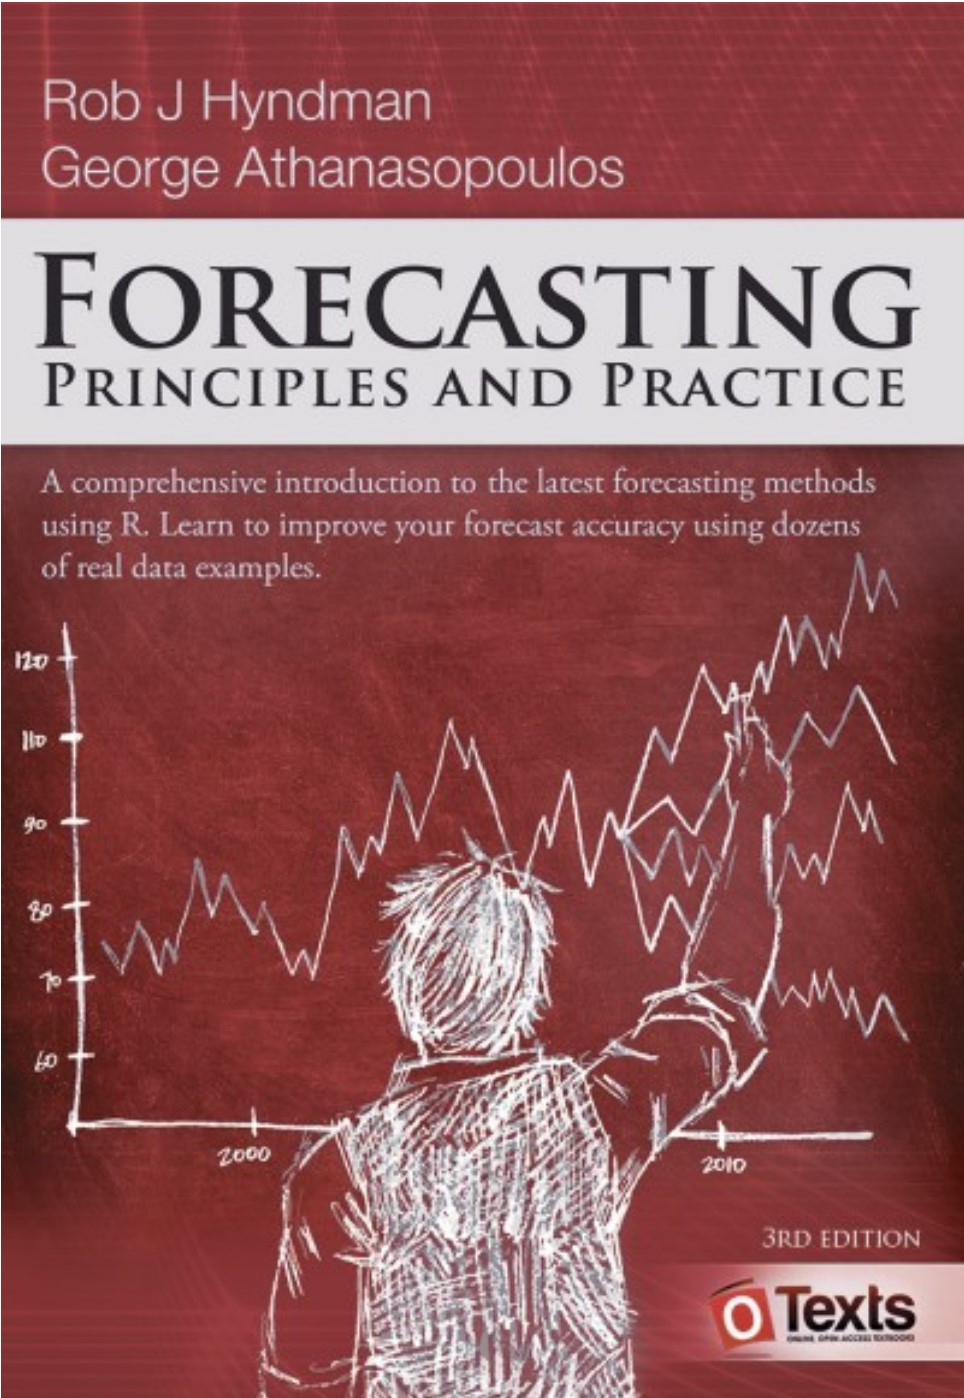
\includegraphics[height=1.2cm, width=1cm]{fpp3_cover}}}] {\scalebox{0.85}{\parbox[t]{1.15\linewidth}{\fullcite{HynAth2021}}}}.
\end{itemize}
\end{frame}

\begin{frame}{Notation}
\phantomsection\label{notation}
\fontsize{14}{15}\sf

\begin{textblock}{8.8}(0.2,1.5)
\centerline{\colorbox[RGB]{210,210,210}{$\bY_{t}=\bS\bm{b}_{t}$}}
\begin{itemize}\tightlist
\item $\by_t=$ vector of all series at time $t$
\item $\bm{b}_t=$ vector of most disaggregated series at time $t$
\item $\bS=$ ``structural matrix'' containing the linear constraints.
\end{itemize}
\only<2>{
\begin{itemize}\tightlist
\item $m$ -- number of bottom-level series
\item $n$ -- number of all series
\end{itemize}}

\end{textblock}

\begin{textblock}{5.7}(11.4,1)
\begin{minipage}{4cm}
\begin{block}{}\centering
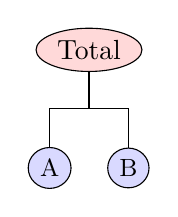
\begin{tikzpicture}
\tikzstyle{every node}=[ellipse,draw,fill=red!15,inner sep=2pt]
\tikzstyle[level distance=.3cm]
\tikzstyle[sibling distance=12cm]
\tikzstyle{level 1}=[sibling distance=10mm,font=\small,set style={{every node}+=[fill=blue!15]}]
\node{Total}[edge from parent fork down]
 child {node {A}
 }
 child {node {B}
 };
\end{tikzpicture}
\end{block}
\end{minipage}
\end{textblock}

\begin{textblock}{5.7}(10.4,3.6)\fontsize{14}{15}\sf
\begin{align*}
\bY_{t}&= \begin{pmatrix}
  y_{\text{Total},t}\\
  y_{A,t}\\
  y_{B,t}
  \end{pmatrix}  \\
  &= \underbrace{\begin{pmatrix}
                1 & 1  \\
                1 & 0  \\
                0 & 1 
                \end{pmatrix}}_{\bS}
     \underbrace{\begin{pmatrix}
       y_{A,t}\\y_{B,t}
       \end{pmatrix}}_{\bm{b}_{t}}
\end{align*}
\end{textblock}
\end{frame}

\begin{frame}{The coherent subspace}
\phantomsection\label{the-coherent-subspace}
\begin{textblock}{9}(.2,1)\fontsize{13}{13}\sf
\begin{block}{Hierarchical time series}
Multivariate time series $\bm{y}_t \in \mathbb{R}^n$, bound by linear contstraints.
\end{block}\vspace*{-0.3cm}
\begin{block}{Coherent subspace}
$m$-dimensional linear subspace $\mathfrak{s}\subset \mathbb{R}^n$ for which linear constraints hold for all $\bm{y}_t\in\mathfrak{s}$.
\end{block}\vspace*{-0.3cm}
\only<2-4>{
\begin{block}{Coherent point forecasts}
$\textcolor{red}{\tilde{\bm{y}}_{T+h|T}}$ is \emph{coherent} if $\textcolor{red}{\tilde{\bm{y}}_{T+h|T}} \in \mathfrak{s}$.
\end{block}}\vspace*{-0.2cm}
\end{textblock}
\only<3-4>{\begin{textblock}{7.5}(.2,6.55)\fontsize{13}{13}\sf
\begin{alertblock}{Base forecasts}
Let $\textcolor{blue}{\hat{\bm{y}}_{T+h|T}}$ be vector of \emph{incoherent} initial $h$-step forecasts.$\phantom{y_{t|h}}$
\end{alertblock}
\end{textblock}}
\only<4>{\begin{textblock}{7.5}(8.3,6.55)\fontsize{13}{13}\sf
\begin{alertblock}{Reconciled forecasts}
Let $\bm{SG}$ be a projection matrix. $\textcolor{red}{\tilde{\bm{y}}_{T+h|T}}=\bm{SG}\textcolor{blue}{\hat{\bm{y}}_{T+h|T}}$ ``reconciles'' $\textcolor{blue}{\hat{\bm{y}}_{T+h|T}}$.
\end{alertblock}
\end{textblock}}

\placefig{9.4}{.0}{width=6.6cm}{3D_hierarchy}
\begin{textblock}{3}(11.4,5.6)\fontsize{13}{13}\sf
\begin{block}{}
\centerline{$y_{Tot} = y_A + y_B$}
\end{block}
\end{textblock}
\end{frame}

\begin{frame}{Geometry of forecast reconciliation}
\phantomsection\label{geometry-of-forecast-reconciliation}
\only<1>{
\begin{textblock}{7}(9.5,1.2)
\resizebox{\textwidth}{!}{\input figs/2D_schematic.tex}
\end{textblock}
}

\only<2->{
\begin{textblock}{9.6}(0.2,0.9)\fontsize{13}{14}\sf
\begin{block}{Reconciled point forecasts}
Let $\psi$ be a mapping, $\psi:\mathbb{R}^n\rightarrow\mathfrak{s}$.  The point forecast $\textcolor{red}{\tilde{\bm{y}}_{T+h|T}}=\psi\left(\textcolor{blue}{\hat{\bm{y}}_{T+h|T}}\right)$ ``reconciles'' a base forecast $\textcolor{blue}{\hat{\bm{y}}_{T+h|T}}$ with respect to the mapping $\psi(.)$
\end{block}\vspace*{-0.2cm}
\end{textblock}
}

\only<2>{
\begin{textblock}{7}(9.5,1.2)
\resizebox{\textwidth}{!}{\input figs/orth_mindistance_schematic.tex}
\end{textblock}
}

\only<3->{
\begin{textblock}{9.7}(0.2,3.67)\fontsize{13}{14}\sf
\begin{block}{Orthogonal Projection}
$\textcolor{red}{\tilde{\bm{y}}_{T+h|T}}=\bm{SG}\textcolor{blue}{\hat{\bm{y}}_{T+h|T}}$ where $\bm{G}=\left(\bm{S}'\bm{S}\right)^{-1}\bm{S}'$ guarantees \vspace*{-0.2cm}
        \begin{equation*} \|(\bm{y}_{t+h}-\textcolor{red}{\tilde{\bm{y}}_{T+h|T}})\|\le\|(\bm{y}_{t+h}-\textcolor{blue}{\hat{\bm{y}}_{T+h|T}})\|
        \end{equation*}
\end{block}\vspace*{-0.2cm}
\end{textblock}
}

\only<3>{
\begin{textblock}{7}(9.5,1.2)
\resizebox{\textwidth}{!}{\input figs/orth_mindistance_schematic1.tex}
\end{textblock}
}

\only<4>{
\begin{textblock}{7}(9.5,1.2)
\resizebox{\textwidth}{!}{\input figs/orth_pointforerec_schematic.tex}
\end{textblock}
}

\only<5>{
\begin{textblock}{7}(9.5,1.2)
\resizebox{\textwidth}{!}{\input figs/orth_mindistance_schematic.tex}
\end{textblock}
}

\only<6->{
\begin{textblock}{9.7}(0.2,6.2)\fontsize{13}{14}\sf
\begin{block}{Oblique Projection}
$\textcolor{red}{\tilde{\bm{y}}_{T+h|T}}=\bm{SG}\textcolor{blue}{\hat{\bm{y}}_{T+h|T}}$,  $\bm{G}=\left(\bm{S}'\bm{\Psi}\bm{S}\right)^{-1}\bm{S}'\bm{\Psi}$  achieves \vspace*{-0.2cm}
        \begin{equation*} \|(\bm{y}_{t+h}-\textcolor{red}{\tilde{\bm{y}}_{T+h|T}})\|_{\bm{\Psi}}\le\|(\bm{y}_{t+h}-\textcolor{blue}{\hat{\bm{y}}_{T+h|T}})\|_{\bm{\Psi}}
        \end{equation*}
\end{block}\vspace*{-0.2cm}
\end{textblock}
}

\only<6>{
\begin{textblock}{7}(9,1.2)
\resizebox{\textwidth}{!}{\input figs/InsampDir_1_George.tex}
\end{textblock}
}

\only<7>{
\begin{textblock}{7}(9,1.2)
\resizebox{\textwidth}{!}{\input figs/InsampDir_2_George.tex}
\end{textblock}
}

\only<8>{
\begin{textblock}{7}(9,1.2)
\resizebox{\textwidth}{!}{\input figs/InsampDir_3_George.tex}
\end{textblock}
}

\only<9>{
\begin{textblock}{7}(9,1.2)
\resizebox{\textwidth}{!}{\input figs/OrthProj_George.tex}
\end{textblock}
}

\only<10->{
\begin{textblock}{7}(9,1.2)
\resizebox{\textwidth}{!}{\input figs/ObliqProj_George.tex}
\end{textblock}
}
\end{frame}

\begin{frame}{Minimum trace (MinT) reconciliation}
\phantomsection\label{minimum-trace-mint-reconciliation}
\fontsize{14}{16}\sf

\begin{itemize}
\tightlist
\item
  How to choose the best \(\bm{\Psi}\)? \pause
\item
  Let
  \(\textcolor{blue}{\bm{W}_h} = \var[\by_{T+h} - \textcolor{blue}{\hat{\by}_{T+h|T}} \mid \by_1,\dots,\by_T]\)
  be the covariance matrix of the base forecast errors.
\item
  Then
  \(\textcolor{red}{\bm{V}_h} = \var[\by_{T+h} - \textcolor{red}{\tilde{\by}_{T+h|T}}  \mid \by_1,\dots,\by_T])  = \bm{SG}\bm{W}_h\bm{G}'\bm{S}'\)
  is the covariance matrix of the reconciled forecast errors.\pause
\end{itemize}

\begin{alertblock}{Minimum trace (MinT) reconciliation}
If $\bm{SG}$ is a projection, then trace of $\textcolor{red}{\bm{V}_h}$ is minimized when $\bm{\Psi} = \textcolor{blue}{\bm{W}_h}$, so that
\centerline{$\bm{SG} = \bS(\bS'\bm{W}_h^{-1}\bS)^{-1}\bS'\bm{W}_h^{-1}$}
\end{alertblock}\pause
\vspace*{-0.2cm}

\begin{itemize}
\tightlist
\item
  MinT is \(L_2\) optimal amongst linear unbiased forecasts.
\end{itemize}

\vspace*{10cm}
\end{frame}

\begin{frame}{MinT linear projections}
\phantomsection\label{mint-linear-projections}
\begin{textblock}{5}(7,-0.1)
\begin{block}{}
\centerline{$\textcolor{red}{\tilde{\by}_{T+h|T}}=\bm{SG}\textcolor{blue}{\hat{\by}_{T+h|T}}$}
\end{block}
\end{textblock}

\begin{textblock}{15}(.2,1.2)\fontsize{13}{15}\sf
\begin{itemize}\parskip=0cm
\item How to estimate $\bm{W}_h = \var[\by_{T+h} - \textcolor{blue}{\hat{\by}_{T+h|T}} \mid \by_1,\dots,\by_T]$?
\end{itemize}
\end{textblock}

\only<2>{

\begin{textblock}{14.4}(.5,2.15)
\begin{alertblock}{Reconc.  method \hspace*{0.6cm} $\bm{SG}$}
\begin{tabular}{l@{\hspace*{-0.5cm}}l}
  OLS             & $\bS(\bS'\bS)^{-1}\bS'$ \\[0.1cm]
  WLS(var)        & $\bS(\bS'\bm{\Lambda}_v\bS)^{-1}\bS'\bm{\Lambda}_v$ where $\bm{\Lambda}_v = \text{diag}(\hat{\bm{W}}_1)^{-1}$\\[0.1cm]
  WLS(struct)     & $\bS(\bS'\bm{\Lambda}_s\bS)^{-1}\bS'\bm{\Lambda}_s$ where $\bm{\Lambda}_s = \text{diag}(\bS\bm{1})^{-1}$\\[0.1cm]
  MinT(sample)    & $\bS(\bS'\hat{\bm{W}}_{1}^{-1}\bS)^{-1}\bS' \hat{\bm{W}}_{1}^{-1}$  \\[0.1cm]
  MinT(shrink)\hspace*{2cm}    & $\bS(\bS'\hat{\bm{W}}_{\text{shr}}^{-1}\bS)^{-1}\bS' \hat{\bm{W}}_{\text{shr}}^{-1}$  \\[0.1cm]
\end{tabular}
\end{alertblock}
\end{textblock}

\begin{textblock}{15}(.2,7.15)\fontsize{13}{15}\sf
\begin{itemize}\parskip=0cm
\item $\hat{\bm{W}}_{\text{shr}}$ is shrinkage estimator $\tau \text{diag}(\hat{\bm{W}}_{1})+(1-\tau)\hat{\bm{W}}_{1}$\\ where $\tau$ selected optimally.
\end{itemize}
\end{textblock}
}
\end{frame}

\begin{frame}{MinT and Geometry papers}
\phantomsection\label{mint-and-geometry-papers}
\begin{textblock}{14}(0.9,1.3)
\begin{itemize} \footnotesize
\item[{\raisebox{-1.1cm}[0cm][0cm]{\textcolor{black}{\includegraphics[width=1cm]{JASA}}}}] \fullcite{WicEtAl2019}.
\end{itemize}
\end{textblock}

\begin{textblock}{14}(0.9,5)
\begin{itemize} \footnotesize
\item[{\raisebox{-1.2cm}[0cm][0cm]{\textcolor{black}{
\includegraphics[width=1cm]{IJFcover}}}}] \fullcite{PanEtAl2021_Geometry}
\end{itemize}
\end{textblock}
\end{frame}

\begin{frame}{Probabilistic forecast reconciliation}
\phantomsection\label{probabilistic-forecast-reconciliation}
\begin{textblock}{9.7}(0.2,1)\fontsize{12}{12}\sf
\begin{block}{}
A probability triple $(\mathfrak{s}, \mathscr{F}_{\mathfrak{s}}, \breve{\nu})$ is coherent with the bottom probability triple $(\mathbb{R}^m, \mathscr{F}_{\mathbb{R}^m}, \nu)$, if
\centerline{$\breve{\nu}(s(\mathcal{B})) = \nu(\mathcal{B}) \quad \forall \mathcal{B} \in \mathscr{F}_{\mathbb{R}^m}$}
\end{block}\vspace*{-0.2cm}
\begin{itemize}\tightlist
\item Random draws from coherent distribution must lie on $\mathfrak{s}$.
\item The probability of points not on $\mathfrak{s}$ is zero.
\item The reconciled distribution is a transformation of the base forecast distribution that is coherent on $\mathfrak{s}$.
\end{itemize}
\end{textblock}
\begin{textblock}{7}(9.5,0.5)
\resizebox{\textwidth}{!}{
\input figs/probforerec_schematic.tex
}
\end{textblock}

\begin{textblock}{15.3}(0.6,6.3)
\begin{itemize} \footnotesize
\item[{\raisebox{-1.2cm}[0cm][0cm]{\textcolor{black}{
\includegraphics[width=1cm]{EJORcover}}}}] {\scalebox{0.85}{\parbox[t]{1.15\linewidth}{\fullcite{PanEtAl2023}}}}
\end{itemize}
\end{textblock}
\end{frame}

\section{Improving univariate
forecasts}\label{improving-univariate-forecasts}

\begin{frame}{Temportal reconciliation: monthly data}
\phantomsection\label{temportal-reconciliation-monthly-data}
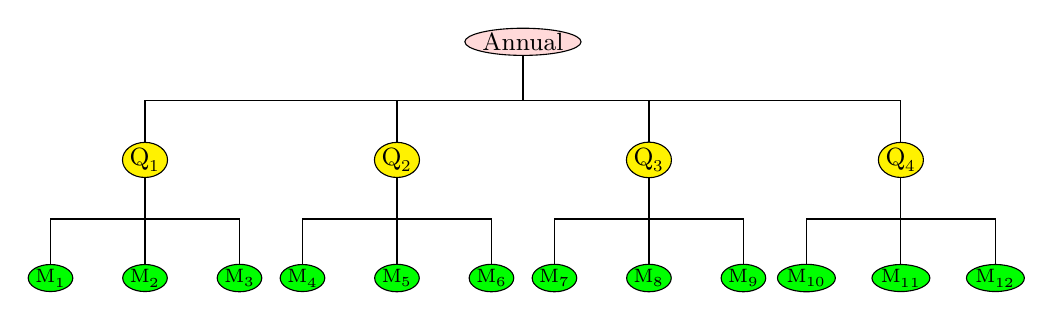
\begin{tikzpicture}
  \tikzstyle{every node}=[ellipse,draw,inner sep=0.2pt,fill=red!15,font=\small]
  \tikzstyle[level distance=.1cm]
  \tikzstyle[sibling distance=7cm]
  \tikzstyle{level 1}=[sibling distance=32mm, set style={{every node}+=[fill=yellow]}]
  \tikzstyle{level 2}=[sibling distance=12mm,font=\scriptsize,set style={{every node}+=[fill=green]}]
  \node{Annual}[edge from parent fork down]
  child {node {Q$_1$}
     child {node {\scriptsize M$_1$}}
     child {node {\scriptsize M$_2$}}
     child {node {\scriptsize M$_3$}}
  }
  child {node {Q$_2$}
      child {node {\scriptsize M$_4$}}
      child {node {\scriptsize M$_5$}}
      child {node {\scriptsize M$_6$}}
  }
  child {node {Q$_3$}
    child {node {\scriptsize M$_7$}}
    child {node {\scriptsize M$_8$}}
    child {node {\scriptsize M$_9$}}
  }
  child {node {Q$_4$}
    child {node {\scriptsize M$_{10}$}}
    child {node {\scriptsize M$_{11}$}}
    child {node {\scriptsize M$_{12}$}}
  };
\end{tikzpicture}

\begin{textblock}{14}(1,6.7)
  \begin{alertblock}{}
    \begin{itemize}
      \item[\color{white}\ding{229}] Forecast series at each available frequency.
      \item[\color{white}\ding{229}] Optimally combine forecasts within the same year.
    \end{itemize}
  \end{alertblock}
\end{textblock}
\end{frame}

\begin{frame}{Example: Accident \& emergency services demand}
\phantomsection\label{example-accident-emergency-services-demand}
\placefig{2}{2.2}{width=0.7\paperwidth}{AEexample.pdf}
\end{frame}

\begin{frame}{Temporal Hierarchical Forecasting - THieF}
\phantomsection\label{temporal-hierarchical-forecasting---thief}
\begin{textblock}{13.5}(0.9,1.4)
\begin{itemize} \footnotesize
\item[{\raisebox{-1.cm}[0cm][0cm]{\textcolor{black}{
\includegraphics[width=1cm]{EJORcover}}}}] \fullcite{AthEtAl2017}
\item[{\raisebox{-1.cm}[0cm][0cm]{\textcolor{black}{
\includegraphics[width=1cm]{EJORcover}}}}] \fullcite{KouAth2021_EJOR}.
\end{itemize}
\end{textblock}
\end{frame}

\section{Improving cross-temporal
forecasts}\label{improving-cross-temporal-forecasts}

\begin{frame}{Cross-temporal reconciliation}
\phantomsection\label{cross-temporal-reconciliation}
\begin{textblock}{6}(0.2,1.2)
\centering\fontsize{12}{13}\sf
\textbf{Geographical division}\\
\includegraphics[width = 5.5cm, trim= 0 0 180 0, clip=true]{figs/aus_map.png}\\[-0.4cm]
\faTimes\\
\textbf{Purpose of travel}\\
{\fontsize{11}{12}\sf Holiday, Visiting friends \& relatives, Business, Other}
\end{textblock}

\begin{textblock}{10}(6.1,1)
\fontsize{11}{14}\sf\tabcolsep=0.12cm
\begin{itemize}
\item \textbf{Cross-sectional aggregations}\newline (geographical divisions $\times$ purpose of travel)

\begin{tabular}{lccccc}
\toprule
  & \textbf{AUS} & \textbf{States} & \textbf{Zones$^\ast$} & \textbf{Regions} & \textbf{Tot}\\
  \midrule
  \textbf{geographical} & 1 & 7 & 21 & 76 & 105 \\
  \textbf{purpose} & 4 & 28 & 84 & {\color{avocado}\textbf{304}} & 420\\
  \midrule
  \textbf{total} & 5 & 35 & 105 & 380 & \textbf{\color{orange}525}\\
  \bottomrule
\end{tabular}
\end{itemize}
\end{textblock}
\only<2->{
\begin{textblock}{9.4}(6.1,6)
\fontsize{11}{14}\sf\tabcolsep=0.12cm
\begin{itemize}
\item \textbf{Temporal aggregations}, frequencies:\\[0.2cm]
\begin{multicols}{2}
  \begin{itemize}\tightlist
  \item Monthly
  \item Bi-Monthly
  \item Quarterly
  \end{itemize}
  \begin{itemize}\tightlist
  \item Four-Monthly
  \item Semi-Annual
  \item Annual
  \end{itemize}
\end{multicols}
\end{itemize}
\end{textblock}
}

\only<3>{
\begin{textblock}{6}(1.2,8)
\alert{Total: 3150 Series}
\end{textblock}
}
\end{frame}

\begin{frame}{Cross-temporal reconciliation}
\phantomsection\label{cross-temporal-reconciliation-1}
\placefig{1.6}{1.2}{width=12.2cm}{figs/CrossTemp.png}
\end{frame}

\begin{frame}{Cross-temporal reconciliation}
\phantomsection\label{cross-temporal-reconciliation-2}
\begin{textblock}{13.5}(0.9,1.7)
\begin{itemize} \footnotesize
\item[{\raisebox{-1.cm}[0cm][0cm]{\textcolor{black}{
\includegraphics[width=1cm]{annals}}}}] {\scalebox{0.85}{\parbox[t]{1.15\linewidth}{\fullcite{KouAth2019}}}}.
\item[{\raisebox{-1.2cm}[0cm][0cm]{\textcolor{black}{
\includegraphics[width=1cm]{IJFcover}}}}] {\scalebox{0.85}{\parbox[t]{1.15\linewidth}{\fullcite{ctprob}}}}.
\item[{\raisebox{-1.2cm}[0cm][0cm]{\textcolor{black}{
\includegraphics[width=1cm]{IJFcover}}}}] {\scalebox{0.85}{\parbox[t]{1.15\linewidth}{\fullcite{hfreview}}}}.
\end{itemize}
\end{textblock}
\end{frame}

\section{Improving multivariate
forecasts}\label{improving-multivariate-forecasts}

\begin{frame}{FLAP (Forecast Linear Augemnted Projection)}
\phantomsection\label{flap-forecast-linear-augemnted-projection}
Intuition:

\begin{itemize}
\tightlist
\item
  Suppose we are interested in multivariate forecasting but do not have
  linear (or non-linear) constraints.
\item
  Can reconciliation help?
\end{itemize}

\pause

\vspace{0.3cm}

\begin{alertblock}{Can we find linear components that:}

\begin{enumerate}
\item are easy to forecast (or easier than the original series);
\item can capture possible common signals;
\item can improve forecasts of original series.
\end{enumerate}

\end{alertblock}
\end{frame}

\begin{frame}{Outline of FLAP Implementation}
\phantomsection\label{outline-of-flap-implementation}
\begin{itemize}
\tightlist
\item
  We want to forecast a multivariate series
  \(\bm{y}_t \in \mathbb{R}^m\). \pause
\item
  Construct synthetic linear components \(\bm{c}_t \in \mathbb{R}^p\)
  where \(\bm{c}_t = \bm{\Phi}\bm{y}_t\). \pause The choice of
  \(\bm{\Phi}\) is arbitrary. \pause
\item
  The augmented vector \((\bm{y}'_t,\bm{c}'_t)' \in \mathbb{R}^m\)
  coheres to known linear constraints. \pause
\item
  Produce forecasts for original series and components
  \(\textcolor{blue}{\hat{\bm{y}}_{t+h}}\) and
  \(\textcolor{blue}{\hat{\bm{c}}_{t+h}}\). \pause
\item
  Project forecasts onto the \(\mathbb{R}^m\) coherent subspace using
  MinT, resulting in \(\textcolor{red}{\tilde{\bm{y}}_{t+h}}\).
\end{itemize}
\end{frame}

\begin{frame}{Geometry of FLAP}
\phantomsection\label{geometry-of-flap}
\only<1>{\placefig{2.3}{1.9}{trim = 0 0 0 20, page=1, height=8.4cm}{figs/FLAP_geometry.pdf}}
\only<2>{\placefig{2.3}{1.9}{trim = 0 0 0 20, page=2, height=8.4cm}{figs/FLAP_geometry.pdf}}
\only<3>{\placefig{2.3}{1.9}{trim = 0 0 0 20, page=3, height=8.4cm}{figs/FLAP_geometry.pdf}}
\only<4>{\placefig{2.3}{1.9}{trim = 0 0 0 20, page=4, height=8.4cm}{figs/FLAP_geometry.pdf}}
\only<5>{\placefig{2.3}{1.9}{trim = 0 0 0 20, page=5, height=8.4cm}{figs/FLAP_geometry.pdf}}
\end{frame}

\begin{frame}{Key results based on MinT}
\phantomsection\label{key-results-based-on-mint}
\begin{enumerate}
\tightlist
\item
  The forecast error variance is \textbf{reduced} with FLAP

  \begin{itemize}
  \tightlist
  \item
    \(\Var(\bm{y}_{t+h} - \textcolor{blue}{\hat{\bm{y}}_{t+h}}) -\Var(\bm{y}_{t+h} - \textcolor{red}{\tilde{\bm{y}}_{t+h}})\)
    is also \textbf{positive semi-definite}. \pause
  \end{itemize}
\end{enumerate}

\vspace*{0.3cm}

\begin{enumerate}
\setcounter{enumi}{1}
\tightlist
\item
  The forecast error variance \textbf{monotonically} decreases with
  increasing number of components

  \begin{itemize}
  \tightlist
  \item
    the diagonal elements of
    \(\Var(\bm{y}_{t+h} - \textcolor{blue}{\hat{\bm{y}}_{t+h}}) -\Var(\bm{y}_{t+h} - \textcolor{red}{\tilde{\bm{y}}_{t+h}})\)
    are non-decreasing as the number of components increases. \pause
  \end{itemize}
\end{enumerate}

\vspace*{0.3cm}

\begin{enumerate}
\setcounter{enumi}{2}
\tightlist
\item
  The forecast projection is \textbf{optimal} to achieve minimum
  forecast error variance for each series.
\end{enumerate}
\end{frame}

\begin{frame}{No free lunch}
\phantomsection\label{no-free-lunch}
\begin{itemize}
\tightlist
\item
  In practice we need to estimate
  \(\bm{W}_h = \Var(\bm{z}_{t+h} - \textcolor{blue}{\hat{\bm{z}}_{t+h})}\).
\item
  Theory works with known \(\bm{W}_h\). \pause 
\item
  The quality of covariance matrix estimates deteriorate with higher
  dimension.\pause
\item
  However for finite dimension, the benefit of FLAP outweighs errors in
  estimating covariance matrix.
\end{itemize}
\end{frame}

\begin{frame}[fragile]{Monthly Australian regional tourism}
\phantomsection\label{monthly-australian-regional-tourism}
\begin{itemize}
\item
  Monthly Australian tourism data by region giving 77 series, from Jan
  1998 to Dec 2019
\item
  Use expanding window time series cross-validation with \(T=84\)
  observations in first training set, and forecast horizons
  \(h=1,2,\dots,12\).
\item
  Estimate \texttt{ets()} models using the \texttt{forecast} package.
\end{itemize}
\end{frame}

\begin{frame}{Monthly Australian regional tourism}
\phantomsection\label{monthly-australian-regional-tourism-1}
\pandocbounded{\includegraphics[keepaspectratio]{subspace_projections_files/figure-beamer/series-1.pdf}}
\end{frame}

\begin{frame}{Monthly Australian regional tourism}
\phantomsection\label{monthly-australian-regional-tourism-2}
\pandocbounded{\includegraphics[keepaspectratio]{subspace_projections_files/figure-beamer/components-1.pdf}}
\end{frame}

\begin{frame}{Monthly Australian regional tourism - \texttt{ets()}}
\phantomsection\label{monthly-australian-regional-tourism---ets}
\pandocbounded{\includegraphics[keepaspectratio]{subspace_projections_files/figure-beamer/visnights-1.pdf}}
\end{frame}

\begin{frame}{FRED-MD}
\phantomsection\label{fred-md}
\begin{itemize}
\item
  Monthly data of macroeconomic variables (McCracken and Ng, 2016).
\item
  Data from Jan 1959 -- Sep 2023. 777 observations on 122 series.
\item
  Same cleaning process as per McCracken and Ng (2016).
\item
  All series scaled to have mean 0 and variance 1.
\item
  Expanding time series cross-validation with initial size of 25 years
  and forecast horizon 12 months.
\end{itemize}
\end{frame}

\begin{frame}{FRED-MD}
\phantomsection\label{fred-md-1}
\pandocbounded{\includegraphics[keepaspectratio]{subspace_projections_files/figure-beamer/fred-md-arima-1.pdf}}
\end{frame}

\begin{frame}[fragile]{Working Paper and R Package}
\phantomsection\label{working-paper-and-r-package}
\fontsize{10}{8}\sf

\fullcite{flap}

\fontsize{12}{8}\sf

You can install the stable version from CRAN

\begin{Shaded}
\begin{Highlighting}[]
\DocumentationTok{\#\# CRAN.R{-}project.org/package=flap}
\FunctionTok{install.packages}\NormalTok{(}\StringTok{"flap"}\NormalTok{)}
\end{Highlighting}
\end{Shaded}

or the development version from Github

\begin{Shaded}
\begin{Highlighting}[]
\DocumentationTok{\#\# github.com/FinYang/flap}
\CommentTok{\# install.packages("remotes")}
\NormalTok{remotes}\SpecialCharTok{::}\FunctionTok{install\_github}\NormalTok{(}\StringTok{"FinYang/flap"}\NormalTok{)}
\end{Highlighting}
\end{Shaded}
\end{frame}

\section{Final comments}\label{final-comments}

\begin{frame}{Forecasting: Principles and Practice}
\phantomsection\label{forecasting-principles-and-practice}
\placefig{0}{1.1}{width=16cm}{figs/OTexts.png}
\begin{textblock}{2.8}(12.5,0)\begin{block}{}\tt OTexts.com\end{block}\end{textblock}
\begin{textblock}{3}(1.2,8.16)\begin{block}{}\fontsize{8}{9}\sf 1st ed 2013; 2nd ed 2018\end{block}\end{textblock}
\only<1>{
\begin{textblock}{1.4}(7.5,8.2)\begin{block}{}\fontsize{8}{9}\sf 3rd ed 2021\end{block}\end{textblock}
}
\begin{textblock}{0.6}(13.2,8.2)\begin{block}{}\fontsize{8}{9}\sf 2025\end{block}\end{textblock}

\only<2>{
\placefig{5.42}{1.15}{width=5.1cm}{figs/fppgr.png}
}
\only<2>{
\begin{textblock}{2}(7.2,8.18)\begin{block}{}\fontsize{8}{9}\sf Greek ed 2024\end{block}\end{textblock}
}
\end{frame}

\begin{frame}{Links}
\phantomsection\label{links}
\centering


\includegraphics[width=0.4\linewidth,height=\textheight,keepaspectratio]{jobad_cr.png}
\hspace{1cm}

\includegraphics[width=0.4\linewidth,height=\textheight,keepaspectratio]{keynoteqr.png}

Postdoc opportunity \hspace{2.5cm} Link to slides \hspace{0.5cm}
\end{frame}

\begin{frame}{Thank you to}
\phantomsection\label{thank-you-to}
\placefig{0.2}{1.4}{trim = 0 0 0 0, clip=TRUE, width=2.6cm, height=3.2cm}{Rob}
\placefig{2.7}{1.4}{trim = 0 0 0 0, clip=TRUE, width=2.6cm, height=3.2cm}{tas}
\placefig{5.2}{1.4}{trim = 0 30 30 20, clip=TRUE, width=2.6cm, height=3.2cm}{nikos}
\placefig{7.7}{1.4}{trim = 0 10 0 0, clip=TRUE, width=2.6cm, height=3.2cm}{fotios}
\placefig{10.2}{1.4}{trim = 0 10 0 0, clip=TRUE, width=2.6cm, height=3.2cm}{hanlin}
\placefig{12.7}{1.4}{trim = 0 0 0 30, clip=TRUE, width=2.6cm, height=3.2cm}{tommy}

\placefig{0.4}{5}{trim = 10 45 0 0, clip=TRUE, width=2.6cm, height=3.2cm}{roman}
\placefig{2.9}{5}{trim = 15 0 0 0, clip=TRUE, width=2.6cm, height=3.2cm}{shanika}
\placefig{5.4}{5}{trim = 30 10 30 0, clip=TRUE, width=2.6cm, height=3.2cm}{puwasala}
\placefig{7.9}{5}{trim = 0 40 0 0, clip=TRUE, width=2.6cm, height=3.2cm}{danielegiro}
\placefig{10.4}{5}{trim = 350 50 300 50, clip=TRUE, width=2.6cm, height=3.2cm}{fin}
\placefig{12.9}{5}{trim = 30 0 0 0, clip=TRUE, width=2.6cm, height=3.2cm}{mitch}
\end{frame}

\begin{frame}{Other information}
\phantomsection\label{other-information}
\vspace*{0.5cm}

\textbf{Forecasting: Principles and Practice}
\href{https://otexts.com/fppgr/}{\color{Blue}{https://otexts.com/fppgr/}}
\newline (Thank you to
\href{https://tourism.upatras.gr/nikas_old/}{\color{Blue}{Ioannis Nikas}}
and
\href{https://tourism.upatras.gr/nikas_old/}{\color{Blue}{Athanasios Koutras}})

\vspace*{.4cm}

\textbf{Monash webpage}
\href{https://research.monash.edu/en/persons/george-athanasopoulos}{\color{Blue}{https://research.monash.edu/en/persons/george-athanasopoulos}}

\vspace*{0.4cm}

\alert{Thank you!}

\nocite{AthEtAl2017,ctprob}
\nocite{hfreview,htsgeometry,WicEtAl2019,flap}
\end{frame}


\begin{frame}[allowframebreaks]{}
  \bibliographytrue
  \printbibliography[heading=none]
\end{frame}



\end{document}
